\documentclass{../lab}
\usepackage{ dsfont }
\usepackage{ float }
\usepackage{ booktabs }
\usepackage{ epstopdf }

\name{Timothy Devon Morris \\ Dan Koch \\ Seth Nielsen}
\course{Me En 537}
\term{Fall 2018}
\labnum{1}

\begin{document}

\begin{task}

  We laid down our coordinate frames as shown in the Figure~\ref{Baxter Coordinate}.

  \begin{figure}[H]
    \centering
    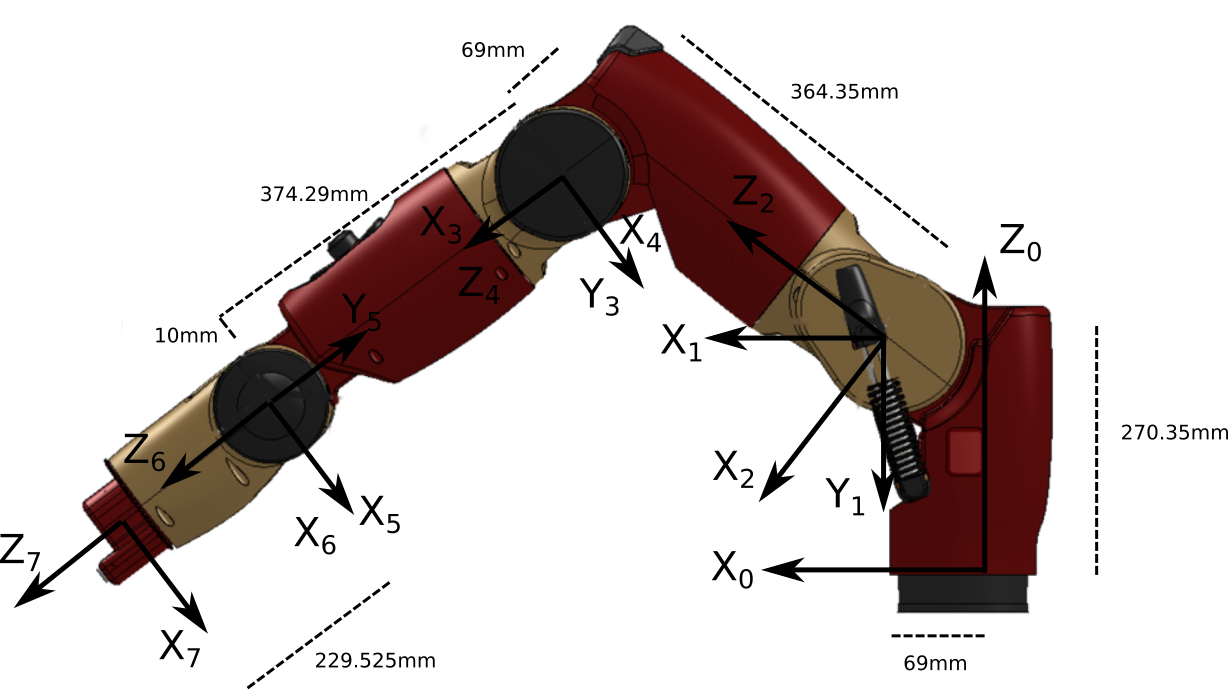
\includegraphics[scale=.4]{baxter.png}
    \label{Baxter Coordinate}
    \caption{Baxter coordinate frames}
  \end{figure}

  With these coordinate frames, we got the DH parameters as shown in Table~\ref{DH}. Note, joint 3 in this figure is not in zero configuration, so the transform between frames 3 and 4 looks strange.

  \begin{table}[H]
    \centering
    \begin{tabular}{|c|c|c|c|r|}
     \hline
     Link & $\theta_i$ & $d_i$ & $a_i$ & $\alpha_i$ \\
     \hline
     1 & $\theta_1$ & .27035 & .069 & $-\pi/2$ \\
     2 & $\theta_2 + \pi/2$ & 0 & 0 & $\pi/2 $\\
     3 & $\theta_3$ & .36435 & .069 & $-\pi/2$ \\
     4 & $\theta_4$ & 0 & 0 & $\pi/2$ \\
     5 & $\theta_5$ & .37429 & .01 & $-\pi/2$ \\
     6 & $\theta_6$ & 0 & 0 & $\pi/2$ \\
     7 & $\theta_7$ & .229525 & 0 & 0 \\
     \hline
    \end{tabular}
  \caption{DH parameters for Baxter}
  \label{DH}
  \end{table}

  Furthermore, we have to premultiply our forward kinematics by the transformation
  \[
    ^{\text{chest}}\xi_0 =
    \begin{bmatrix}
      \cos(\pi/4) & \sin(\pi/4) & 0 & 0.0635 \\
      -\sin(\pi/4) & \cos(\pi/4) & 0 & -0.259 \\
      0 & 0 & 1 & 0.119 \\
      0 & 0 & 0 & 1
    \end{bmatrix}
  \]
  because all our measurements were taken in the chest frame. We then plotted these positions using the Robotics toolbox, as shown below.

  \begin{figure}[H]
    \centering
    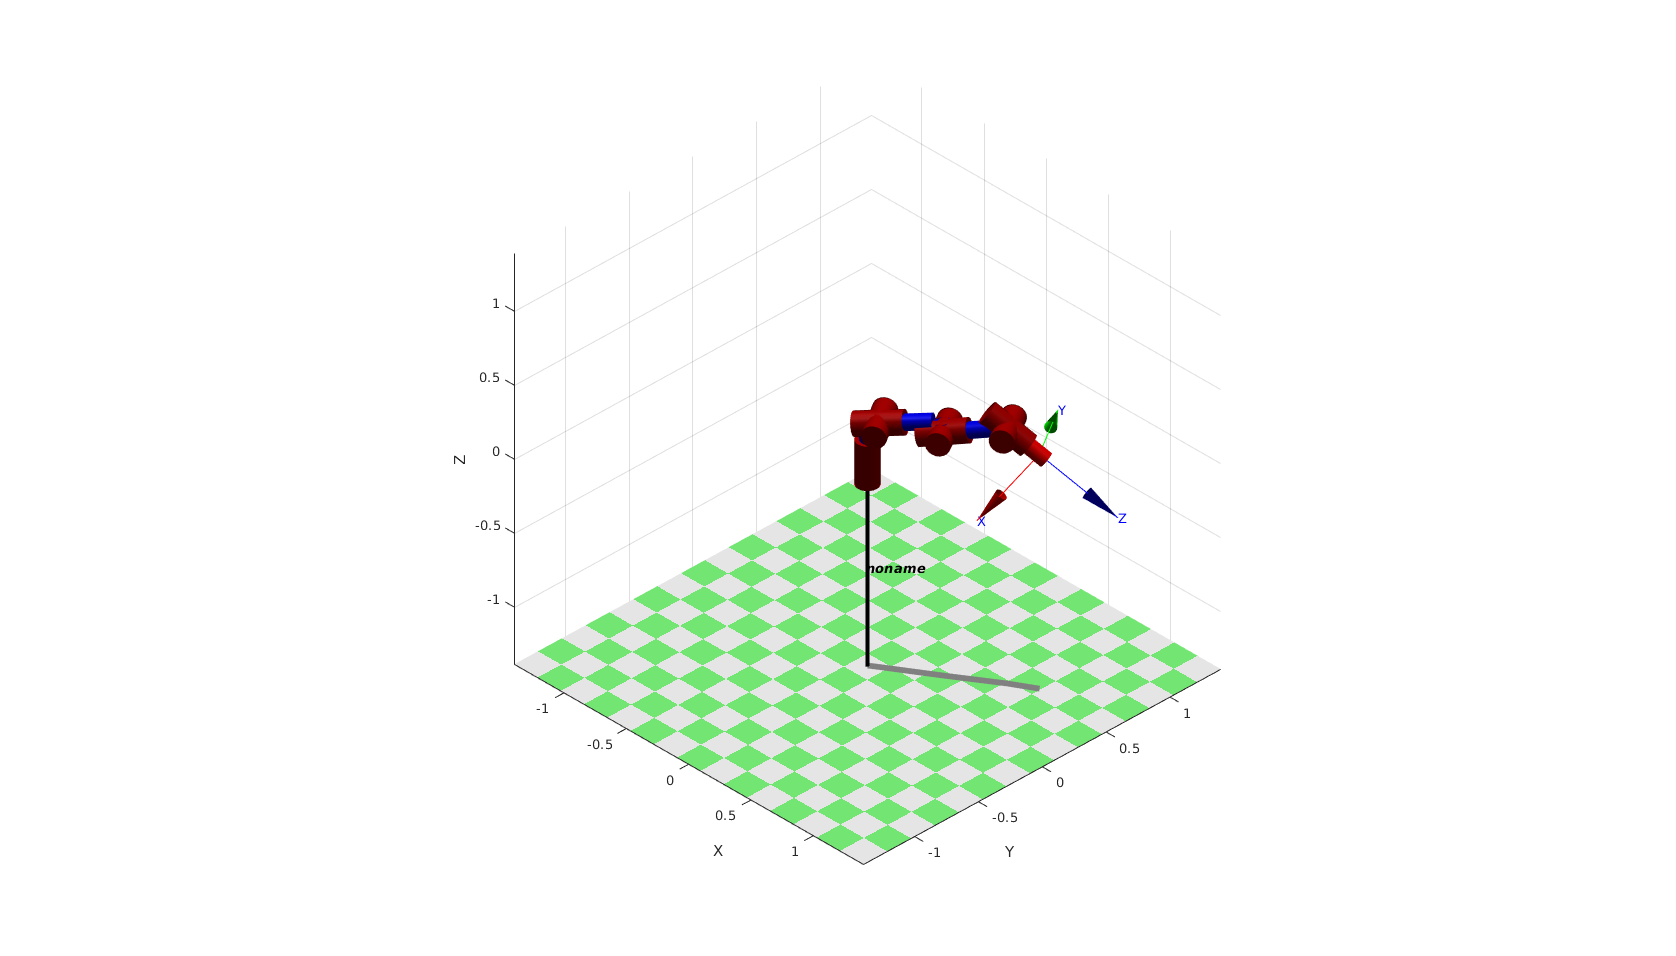
\includegraphics[scale=.3]{task1-1.png}
    \label{Pos1}
    \caption{Position 1}
  \end{figure}

  \begin{figure}[H]
    \centering
    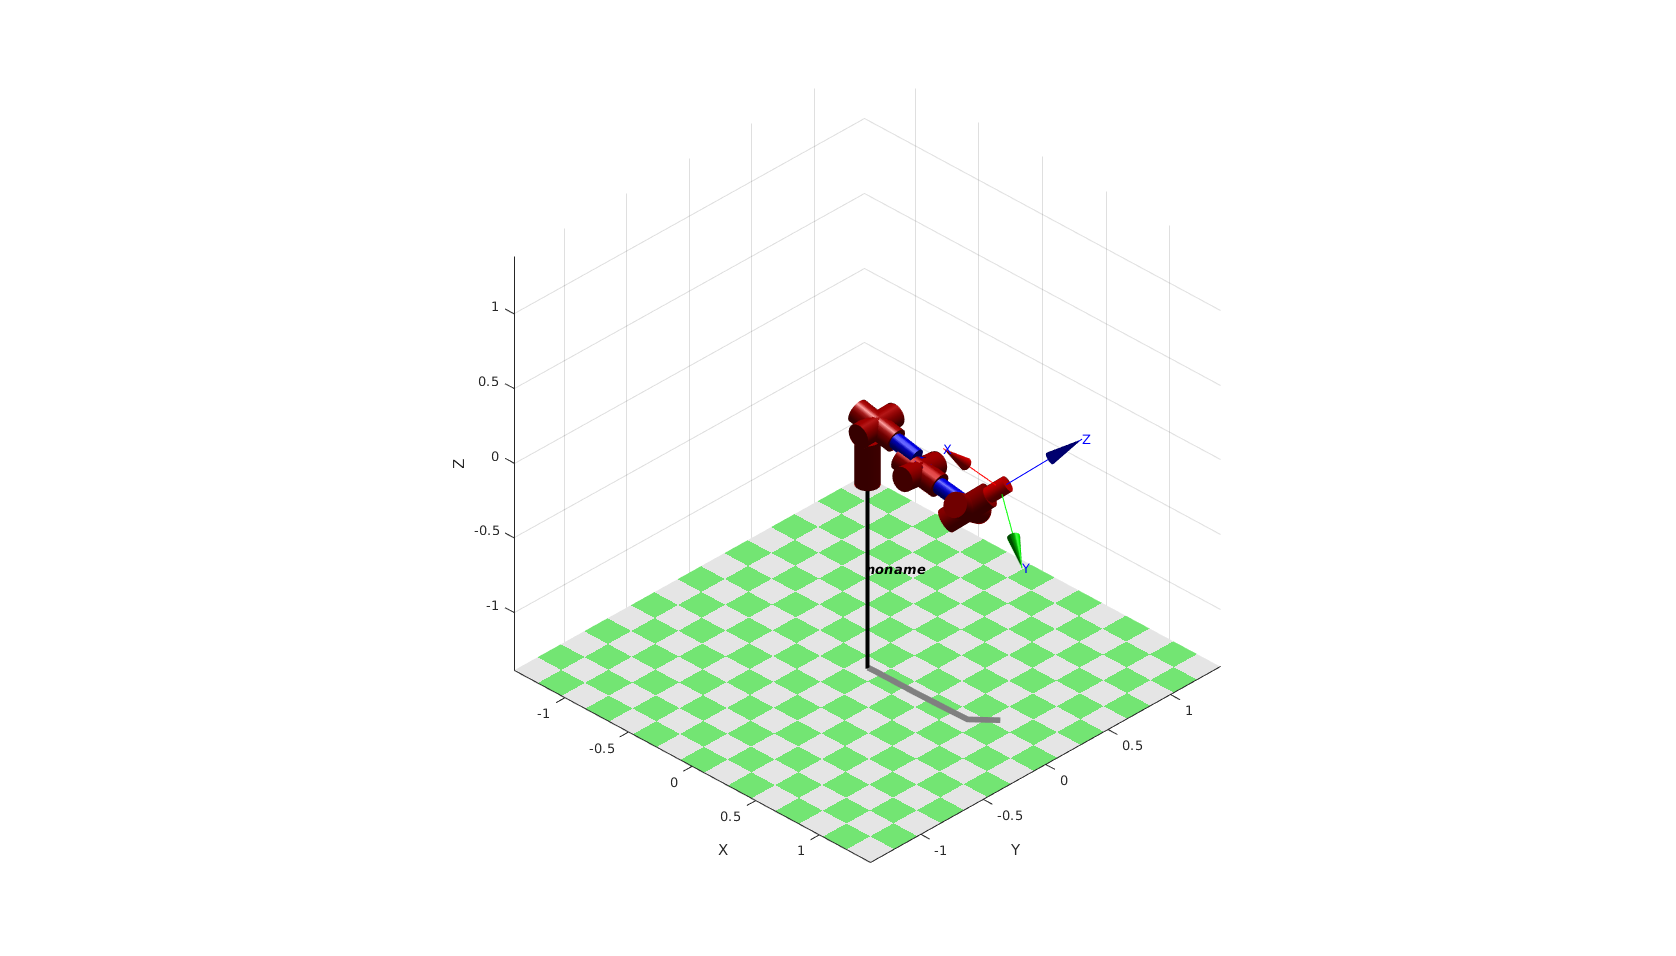
\includegraphics[scale=.3]{task1-2.png}
    \label{Pos2}
    \caption{Position 2}
  \end{figure}

  \begin{figure}[H]
    \centering
    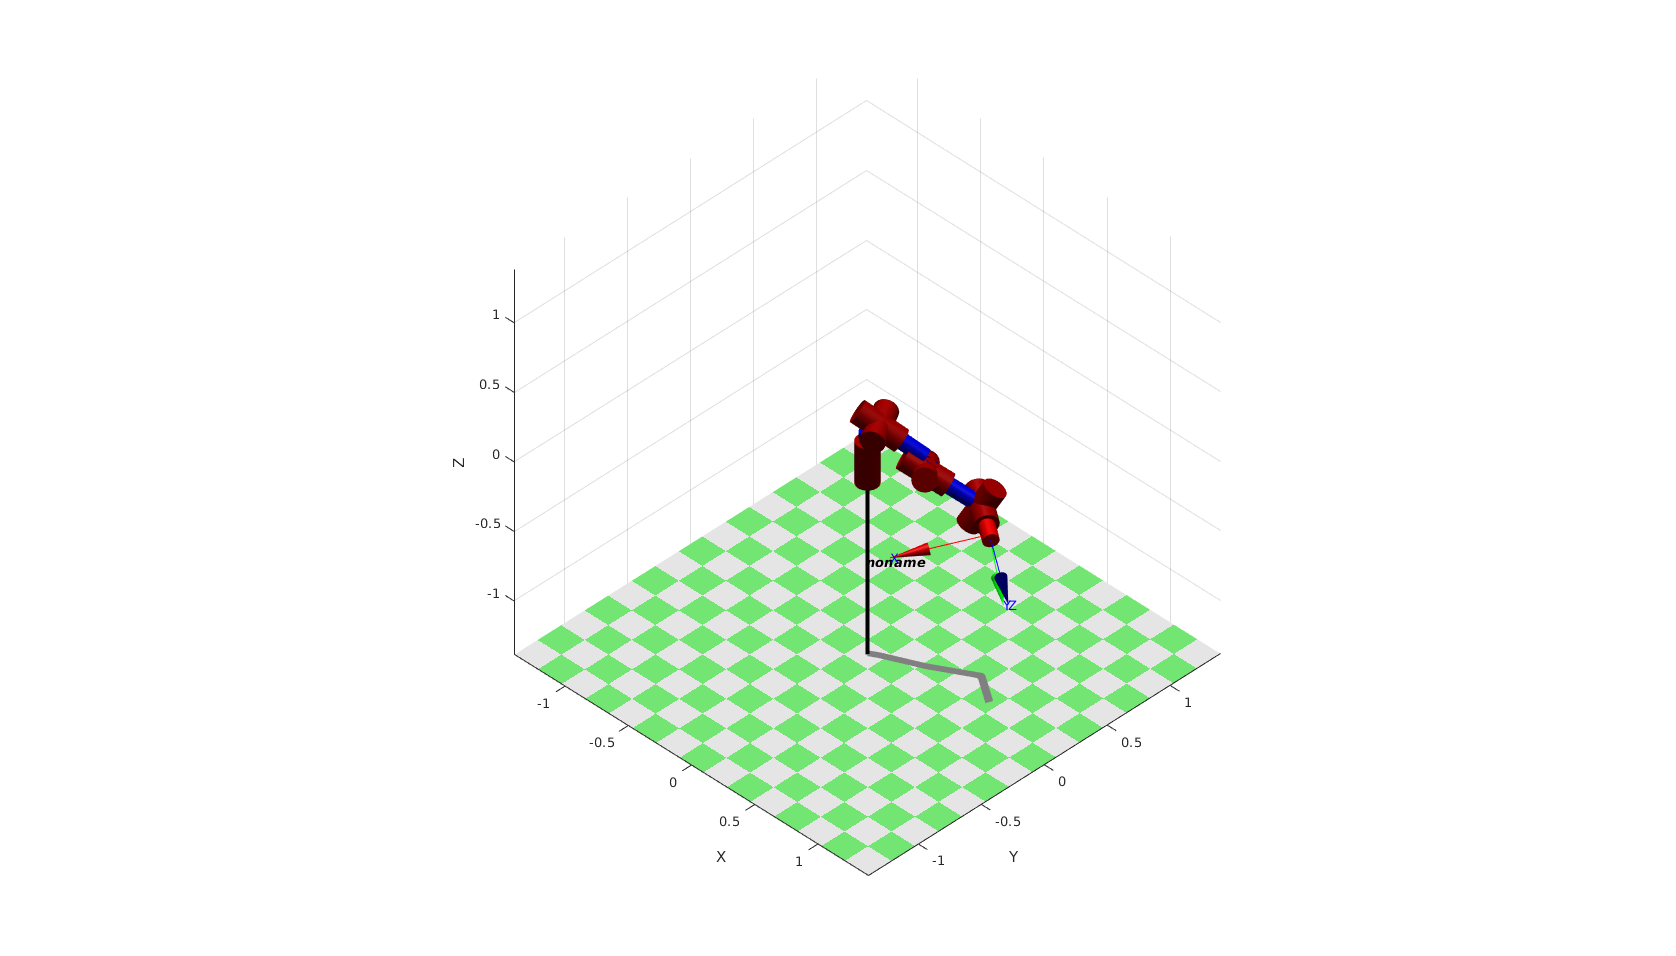
\includegraphics[scale=.3]{task1-3.png}
    \label{Pos3}
    \caption{Position 3}
  \end{figure}

  \begin{figure}[H]
    \centering
    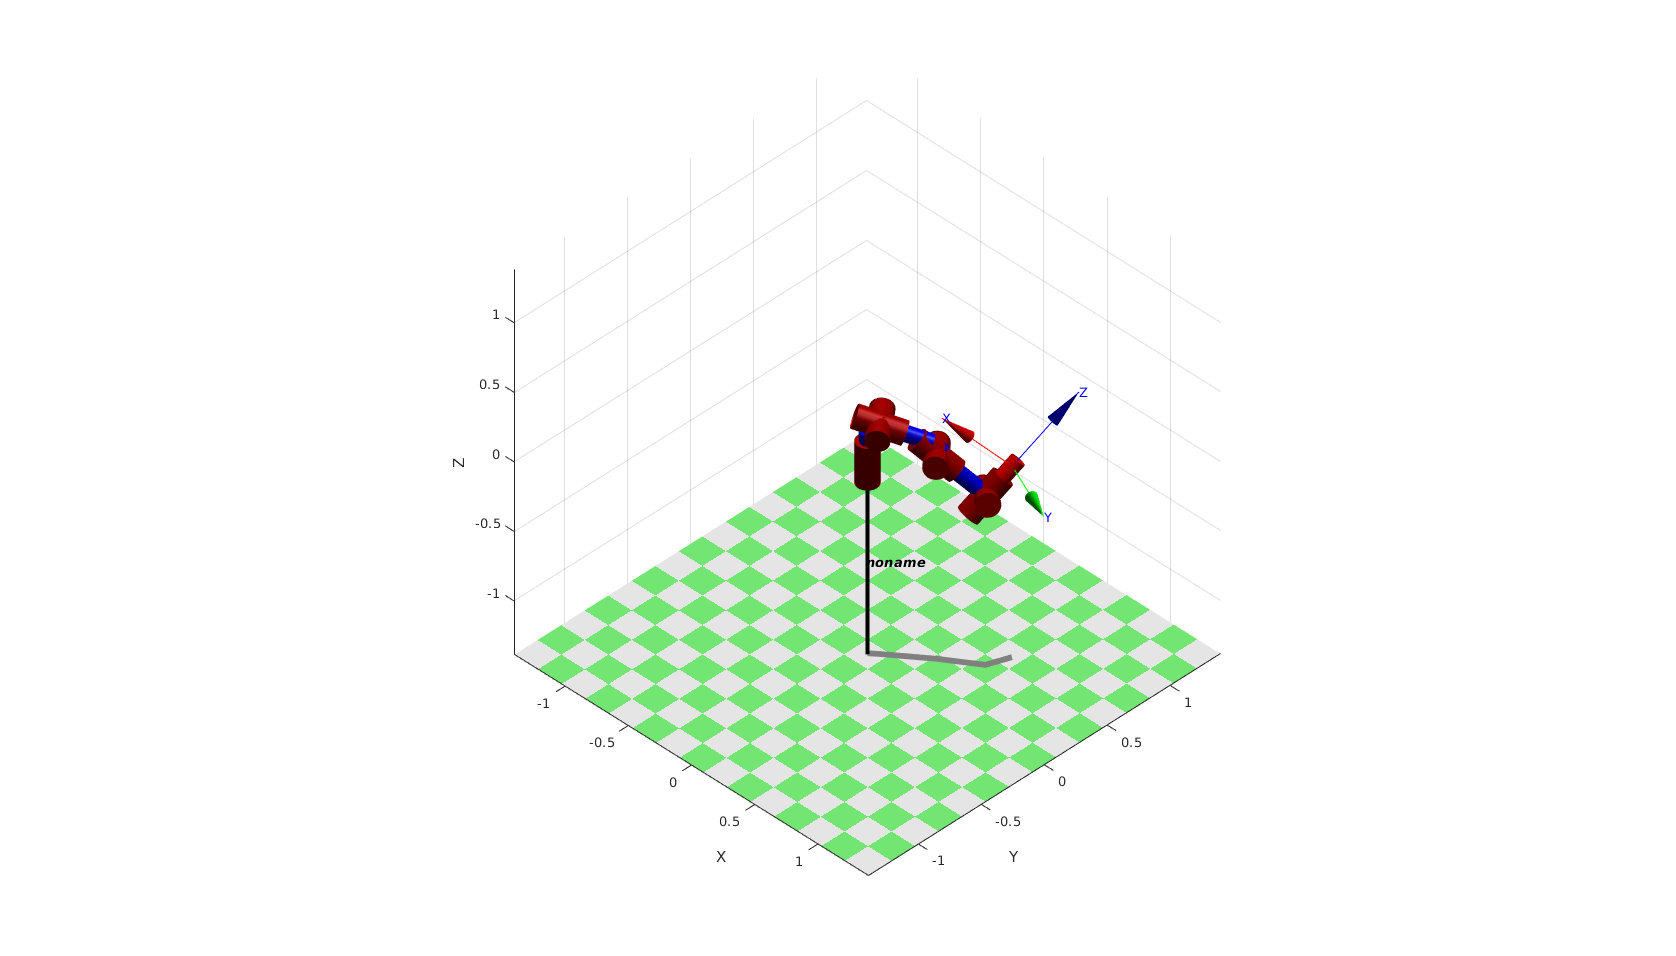
\includegraphics[scale=.3]{task1-4.png}
    \label{Pos4}
    \caption{Position 4}
  \end{figure}
  Now we compare the end effector pose using Matlab's Robotics Toolbox to the measured pose in Table~\ref{predicted}
  \begin{table}[H]
    \hskip-1cm
    \setlength\tabcolsep{0.2cm}
    \begin{tabular}{|c|c|c|c|c|}
     \hline
     & $R_{est}$ & $R_{meas}$ & $p_{est}$ & $p_{meas}$ \\
     \hline
     1 & $
     \begin{bmatrix}
       -.6123 & .1710 & .7719 \\
       .0031 & .9769 & -.2139 \\
       -.7906 & -.1285 & -.5986
   \end{bmatrix}$ &
   $\begin{bmatrix}
       -.6155 & .1723 & .7690 \\
       .0020 & .9761 & .2170 \\
       -.7881 & -0.1320 & -0.6012
   \end{bmatrix}$ & 
   $ \begin{bmatrix}
     1.0291 \\
     -0.4791 \\
     0.3234
   \end{bmatrix} $ &
   $\begin{bmatrix}
    1.0298 \\
    -0.4809 \\
    0.3206
   \end{bmatrix}$
     \\
     2 &
   $\begin{bmatrix}
     -.5621 & .2059 & .8010 \\
     -.3950 & -.9178 & -.0413 \\
     .7267 & -.3396 & .5972
   \end{bmatrix}$ &
   $\begin{bmatrix}    
   -.5599 & .2027 & .8034 \\
   -.3918 & -.9191 & -.0411 \\
   .7301 & -.3378 & .5940 \\
 \end{bmatrix}$ &
 $\begin{bmatrix}
   0.8028 \\
   -0.8052 \\
   0.2932
 \end{bmatrix}$ &
 $ \begin{bmatrix}
   0.8026 \\
   -0.8067 \\
   0.2924
 \end{bmatrix}$ \\
 3 & $
 \begin{bmatrix}
   -.9732 & .1372 &  .1847 \\ 
   -.1687 & .1206 & -.9783 \\ 
   -.1565 &-.9832 & -.0943 \\ 
 \end{bmatrix}$ & 
 $ \begin{bmatrix}
 -.9741& .1333& .1825 \\
 -.1673& .1176&-.9789 \\
 -.1520&-.9840&-.0922 \\
 \end{bmatrix} $ &
 $\begin{bmatrix}
  0.7425 \\
  -0.6865 \\
  -0.0637
 \end{bmatrix}$ &
 $\begin{bmatrix}
  0.7437 \\
  -0.6889 \\
  -0.646
 \end{bmatrix}$ \\
 4 & 
 $\begin{bmatrix}
   -0.6895 &  0.3076 &  0.6557  \\ 
   -0.1324 & -0.9436 &  0.3034  \\ 
    0.7121 &  0.1223 &  0.6914  \\ 
  \end{bmatrix}$ & 
  $\begin{bmatrix}
    -0.6868& 0.3063& 0.6592 \\
    -0.1291&-0.9439& 0.3041 \\
     0.7153& 0.1237& 0.6878 \\
   \end{bmatrix}$ & 
   $ \begin{bmatrix}
     0.8743 \\
     -0.2945 \\
     0.1126
   \end{bmatrix}$ &
   $\begin{bmatrix}
     0.8743 \\
     -0.2966 \\
     0.1100
   \end{bmatrix}$ \\
  \hline
    \end{tabular}
  \caption{Predicted and measured end effector poses}
  \label{predicted}
  \end{table}
  We show our error between our estimate and measured pose in Table~\ref{error}
  \begin{table}[H]
    \centering
    \setlength\tabcolsep{0.2cm}
    \begin{tabular}{|c|c|c|c|c|}
     \hline
     & $R_{meas}R_{est}^T$ & $p_{est}$ - $p_{meas}$ \\
     \hline 1 &
     $\begin{bmatrix}
       1.000 & .0019 & .0038 \\
       -.0019 & 1.000 & -.0033 \\
       -.0038 & .0033 & 1.000
     \end{bmatrix}$ &
     $\begin{bmatrix}
       -0.0006 \\
       0.0018 \\
       0.0027
     \end{bmatrix}$ \\
     2 &
     $ \begin{bmatrix}
       1.000 & .0019 & .0041 \\
       -.0019 & 1.000 & -.0028 \\
       -.0041 & .0028 & 1.000
     \end{bmatrix}$ &
     $ \begin{bmatrix}
      0.0002 \\
      0.0015 \\
      0.0008
     \end{bmatrix} $ \\
     3 &
     $ \begin{bmatrix}
       1.000 & .0019 & .0041 \\
       -.0019 & 1.000 & -.0028 \\
       -.0041 & .0028 & 1.000
     \end{bmatrix}$ &
     $ \begin{bmatrix}
      0.0014 \\
      0.0023 \\
      0.0010
     \end{bmatrix} $ \\
     4 &
     $ \begin{bmatrix}
       1.000 & .0019 & .0041 \\
       -.0019 & 1.000 & -.0028 \\
       -.0041 & .0028 & 1.000
     \end{bmatrix}$ &
     $ \begin{bmatrix}
      -0.0001 \\
      0.0021 \\
      0.0026
     \end{bmatrix} $ \\
     \hline
    \end{tabular}
  \caption{Error in end effector estimates}
  \label{error}
  \end{table}

  As seen the error in orientation is practically the identity matrix, meaning that there is very little error in the orientation estimate. Furthermore, the entries in the position estimate are all less than 3mm from the true position.
  The error in these estimates can arise from encoder resolution, encoder slippage (gear backlash) and lack of precision in the lengths of the links in our model. Overall, however, these estimates are very good and the model matches the actual robot to high degree.
\end{task}

\begin{task}
  In this task, we commanded the robot arm to a position and had it return to zero configuration and come back to the desired position. We then measured the height of the end effector above the ground and analyzed its variance. We did this for two different configurations as shown below. 

  \begin{figure}[H]
    \centering
    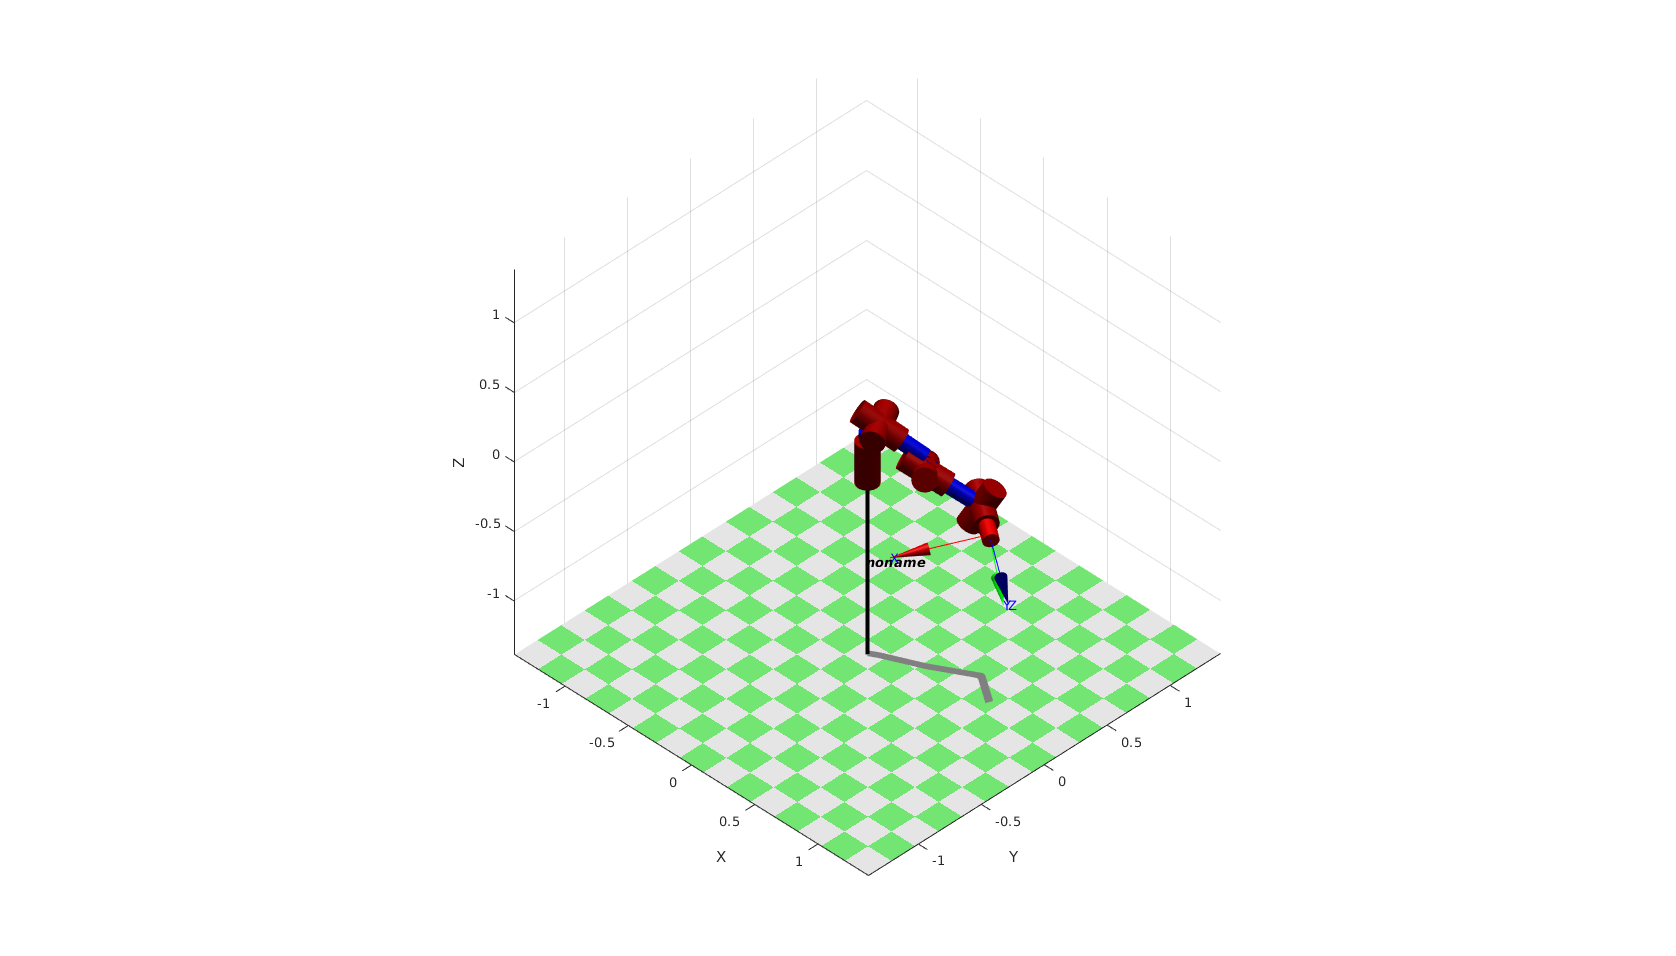
\includegraphics[scale=.3]{task2-1.png}
    \label{t2Pos1}
    \caption{Position 1}
  \end{figure}

  \begin{figure}[H]
    \centering
    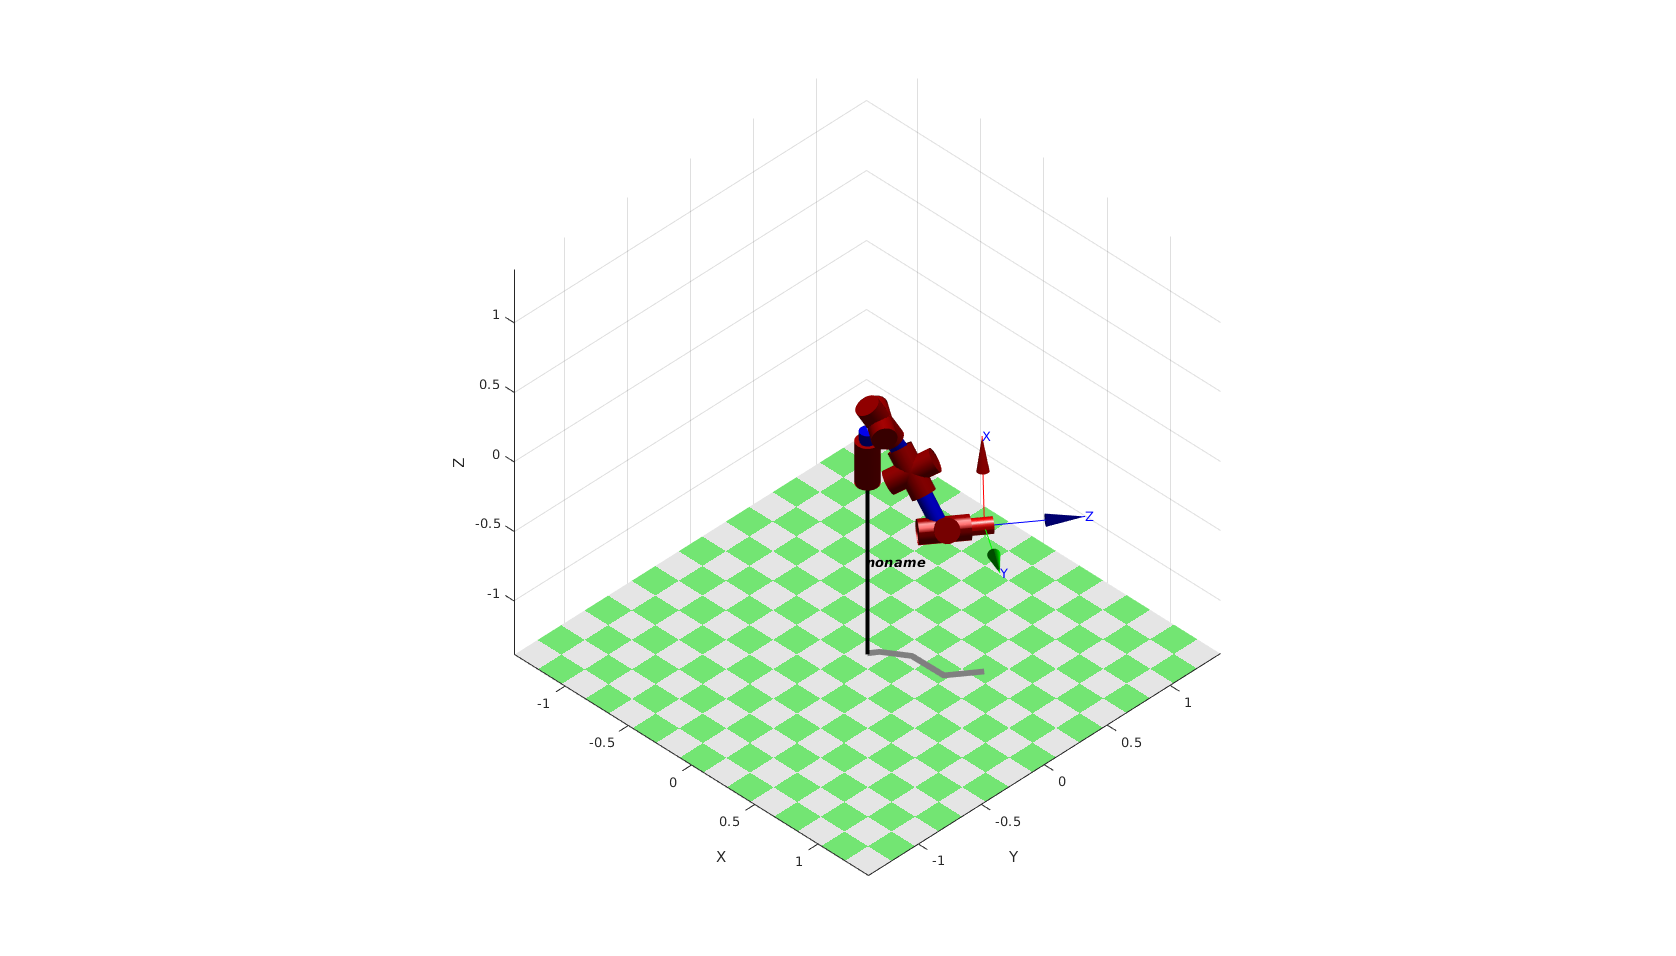
\includegraphics[scale=.3]{task2-2.png}
    \label{t2Pos2}
    \caption{Position 2}
  \end{figure}

  The height above the ground in cm and associated variance are shown in Table~\ref{var}.
  \begin{table}
  \centering
  \setlength\tabcolsep{0.1cm}
  \begin{tabular}{|c|cccccccccc|c|}
    \hline
    Test & & & & & & & & & & & Variance\\
   \hline
   1 & 81.5 & 82.0 & 82.0 & 82.0 & 82.0 & 81.5& 81.5& 81.5& 81.7 & 81.5 & \bf{0.0618} \\
   2 & 71.8 & 71.7 & 71.8 & 71.7 & 71.8 & & & & & & \bf{0.0030} \\
   \hline
  \end{tabular}
  \label{var}
  \caption{Height measurements and variance of end effector}
  \end{table}

  We also analyzed the variance of joint angles as shown in Table~\ref{qvar}.
  \begin{table}[H]
  \centering
  \setlength\tabcolsep{0.1cm}
  \begin{tabular}{|c|ccccccc|}
    \hline
    Joint & 1 & 2 & 3 & 4 & 5 & 6 & 7 \\
   \hline
   Variance ($10^{-5}$ rad) & 0.0151 & 0.0470 & 0.0261 & 0.0127 & 0.0225 & 0.2431 & 0.0163 \\
   \hline
  \end{tabular}
  \label{qvar}
  \caption{Variance of joint angles}
  \end{table}

    There are several possible sources of error in the arm’s vertical positioning that could explain the above results. The resolution of the encoders means that each joint has a small window of undetected rotation between increments in the encoder’s measured angle, which could become significant over the length of seven joints. Overshooting due to momentum of fast moving joints can also cause error in the end effector’s position. The imprecise method of measurement, with a tape measure as the measuring device, is also a source of error.

    Table~\ref{qvar} shows the variances of the recorded joint angles from Test 1. It can be seen from the data that joint 6 had a much higher variance than all other joints, and thus could have a greater contribution to the variance of the vertical measurement, unless its proximity to the end effector mitigated its effect.

    One particularly interesting result is that the variance of the measurements from Test 1 was an order of magnitude greater than for Test 2 (see Table~\ref{var}). Since the only variable between the tests was the pose of the arm, it is likely that the higher precision can be attributed to the change of pose. In Test 2, the end effector was about 20 cm closer to the base frame’s z-axis. This means that for the same joint velocity of the first joints, the end effector moved more slowly in the second pose. This could cause less overshoot in the joint angles and thus increase the robot’s repeatability for that pose. 
  
\end{task}

\begin{task}
  In this task, we picked to positions that were spaced far apart and ran some code that drove the arm between these two poses. Figures \ref{jac1} and \ref{jac2} show the linear and angular velocities of the end effector expressed in the base frame, calculated using the Jacobian. The figures plot the average velocity between the ten trials as a solid blue line, with the dotted black line showing three standard deviations between the three trials. 

  \begin{figure}[H]
    \centering
    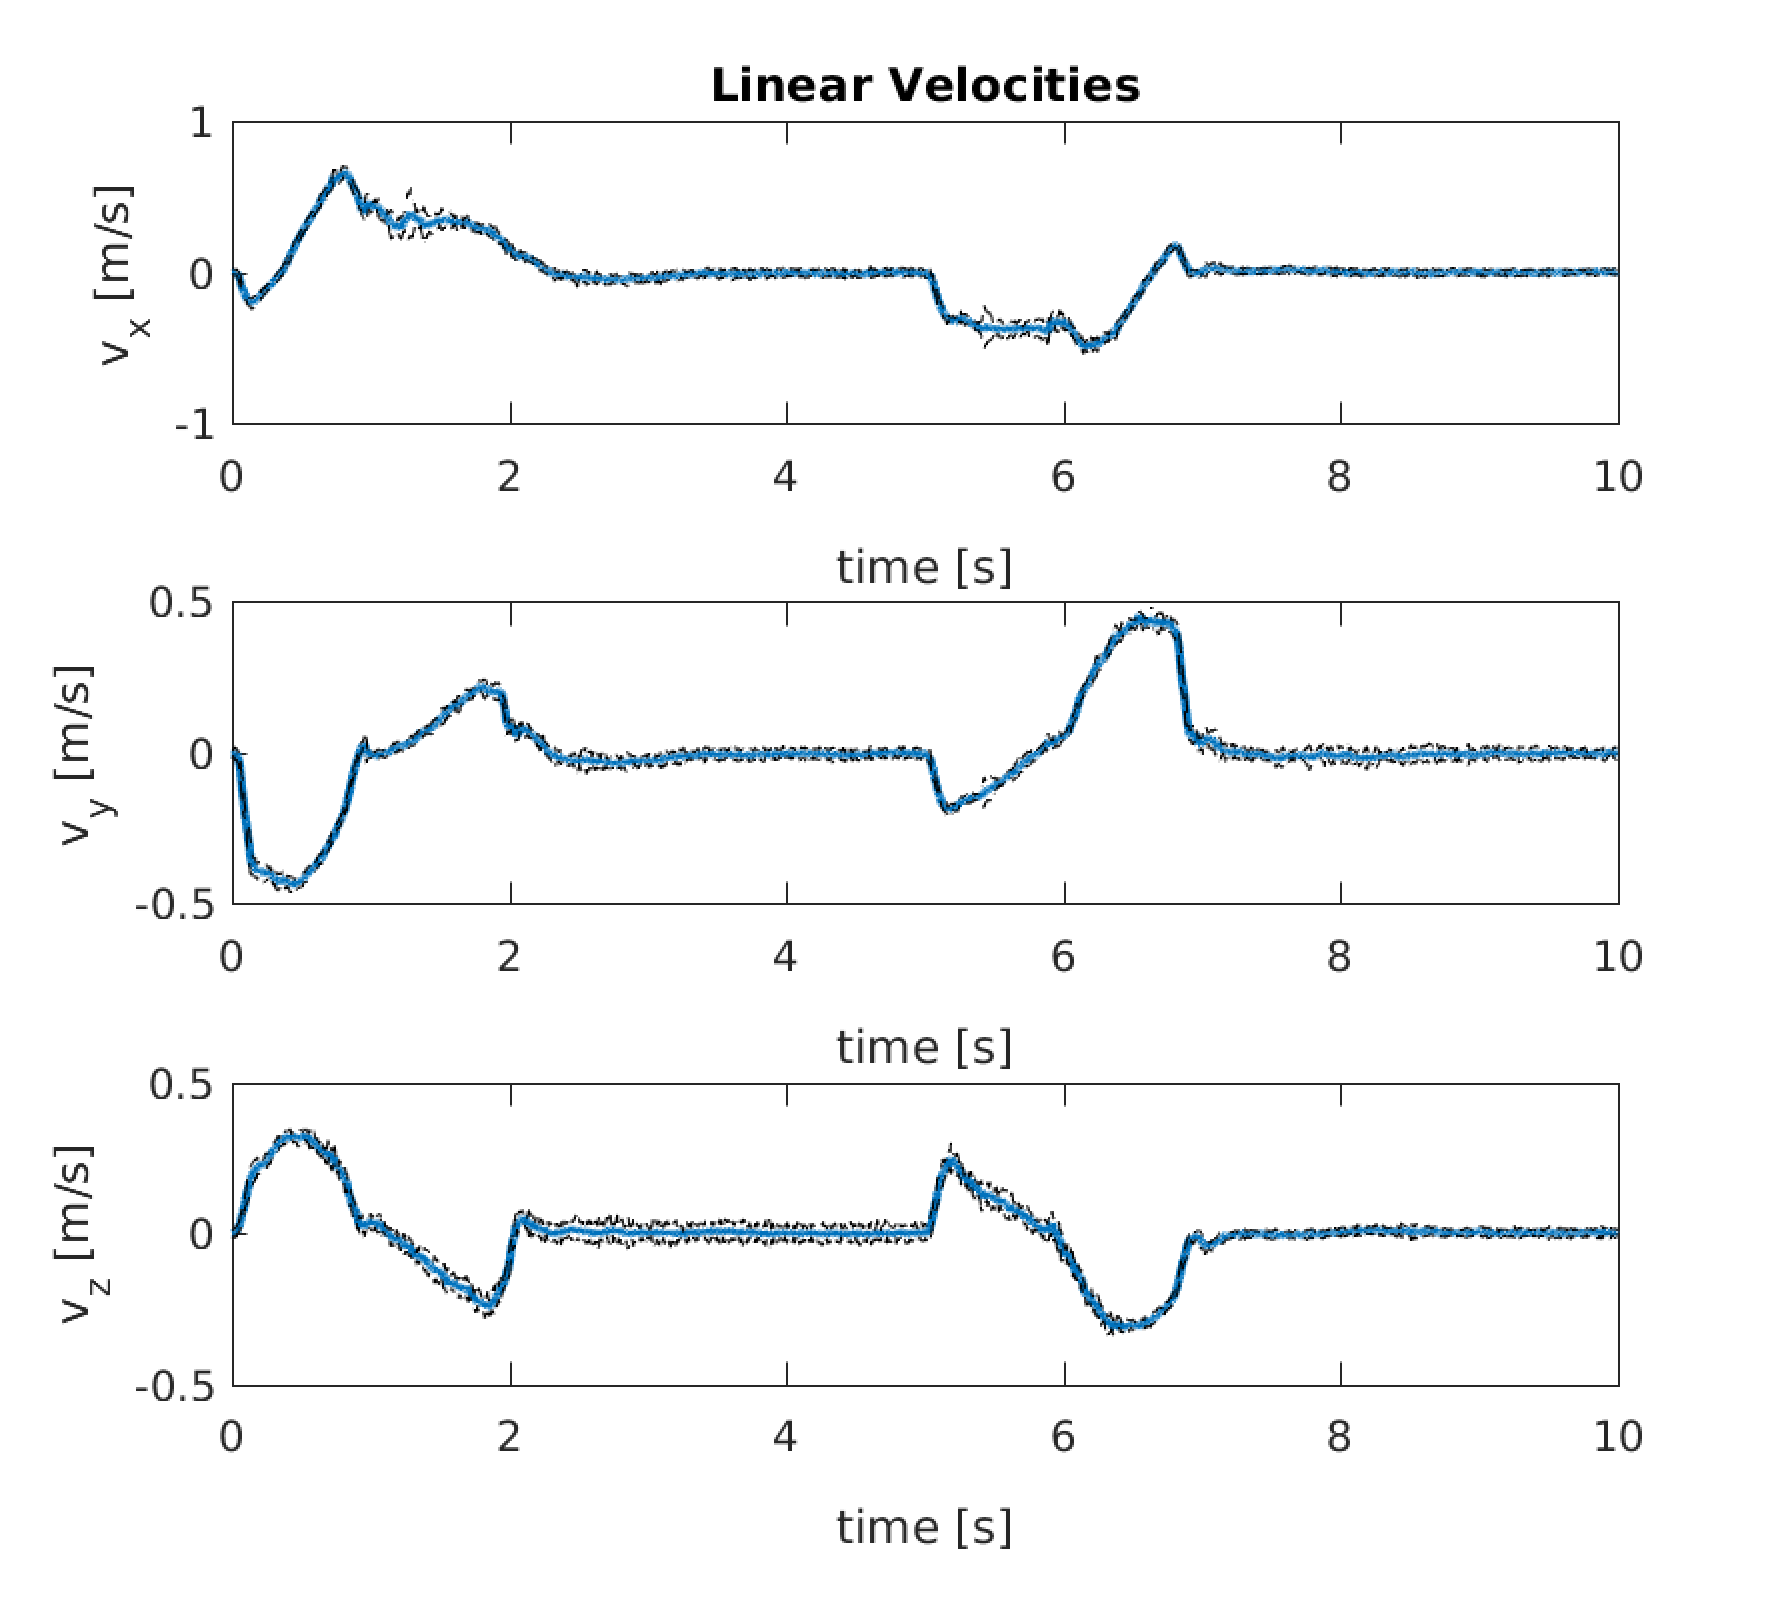
\includegraphics[scale=.2]{linear_vel_avg.png}
    \label{jac1}
    \caption{Linear velocity of end effector}
  \end{figure}

  \begin{figure}[H]
    \centering
    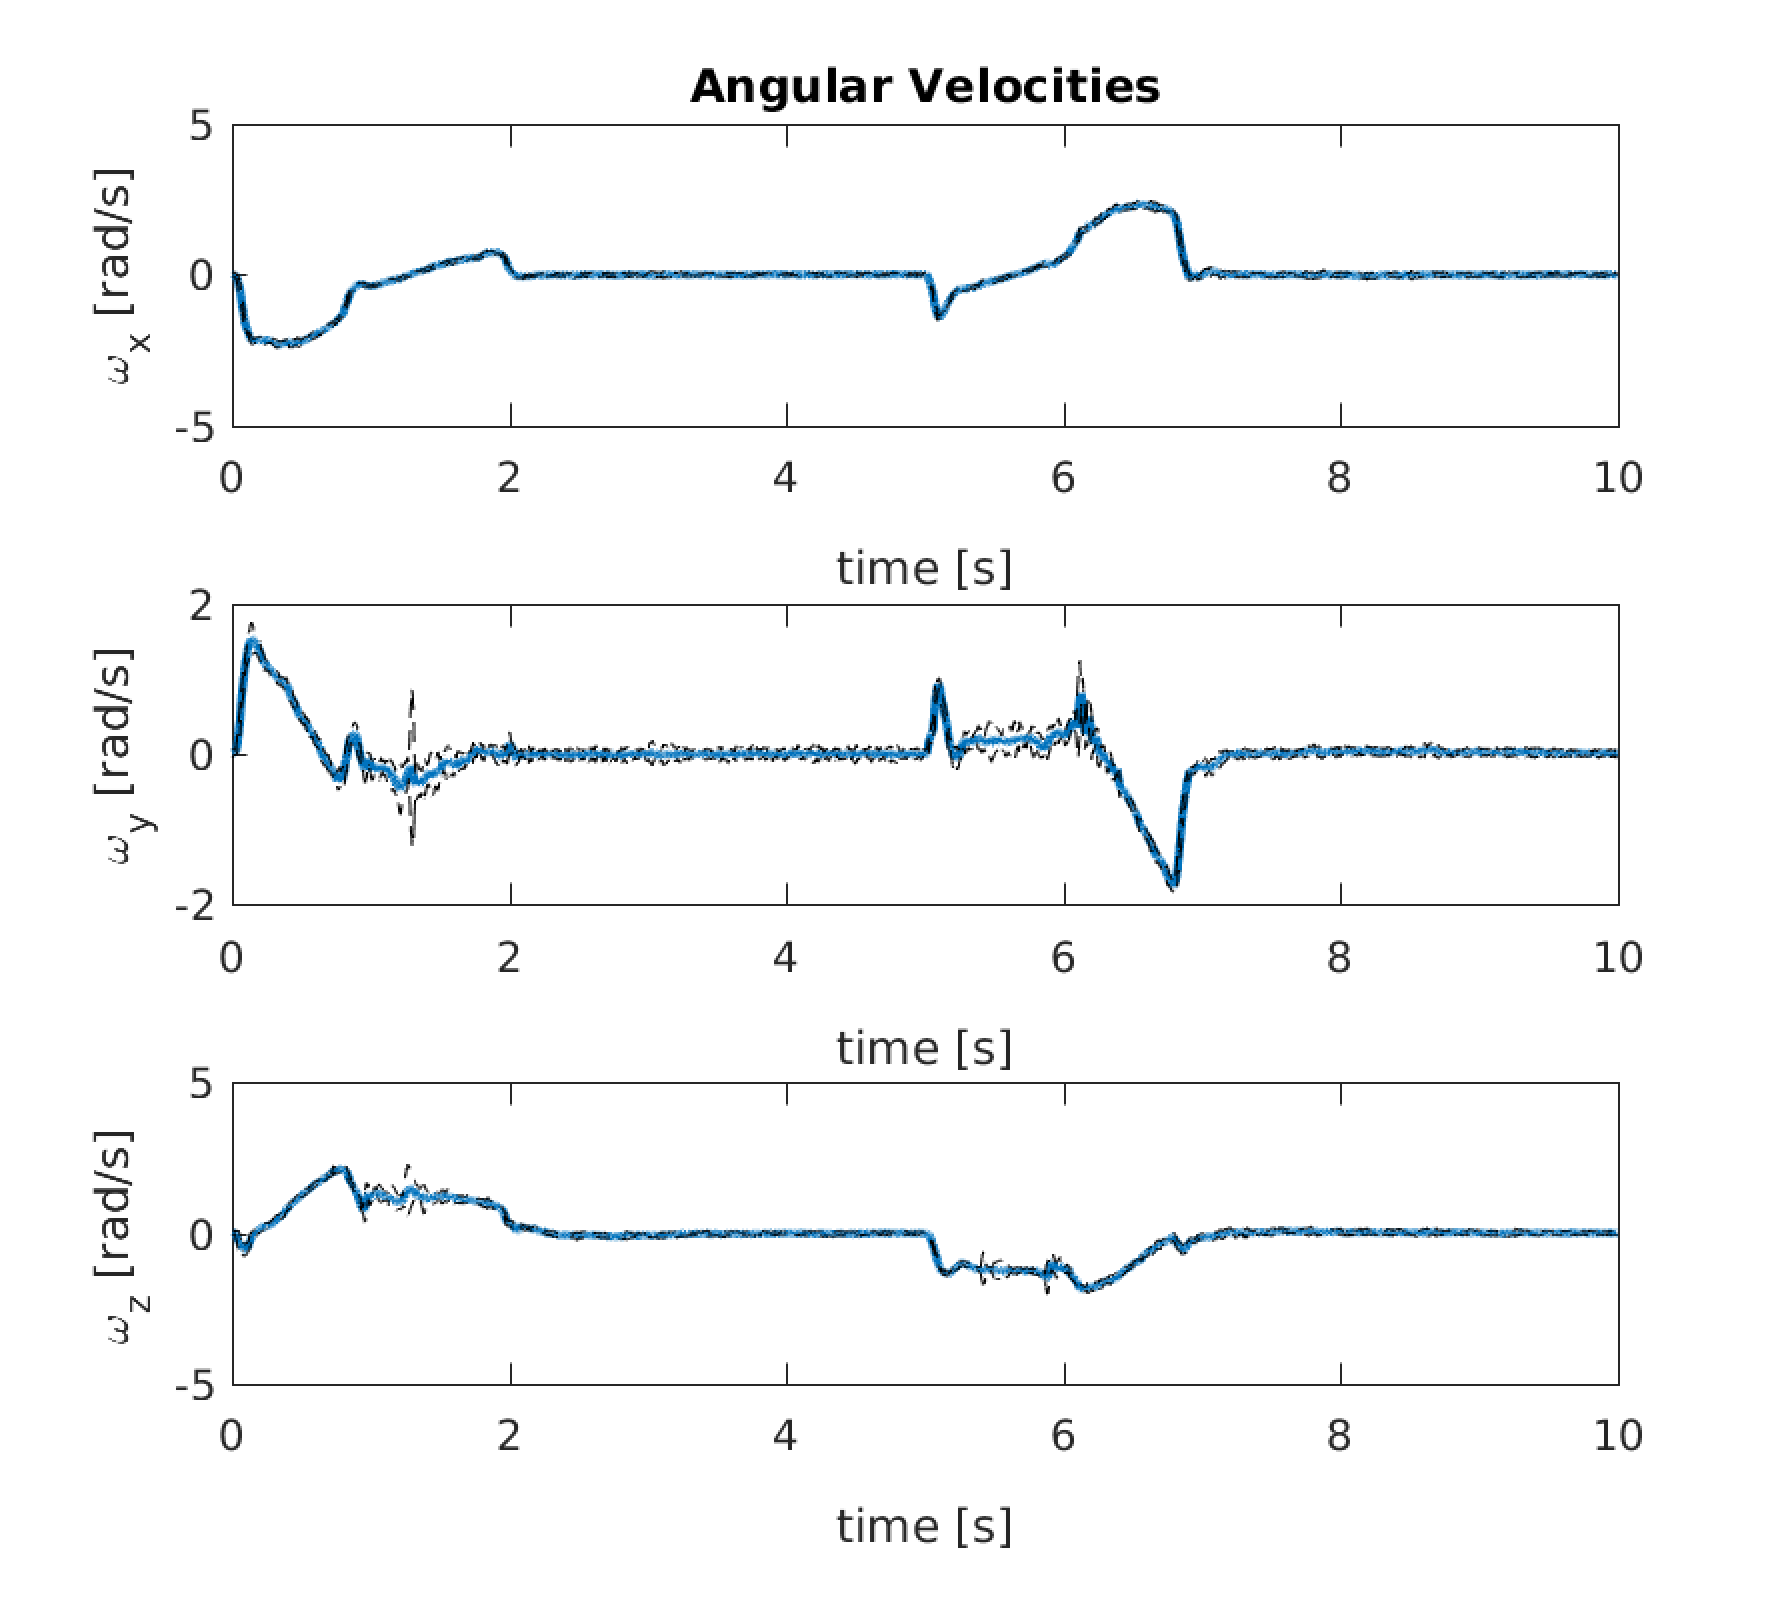
\includegraphics[scale=.2]{angular_vel_avg.png}
    \label{jac2}
    \caption{Angular velocity of end effector}
  \end{figure}

The differences between the velocities in each trial arise probably from three main sources. The first is that since the Baxter robot is not particularly rigid, there will be differences in the response between each trial. The second source of differences arises because the controllers driving the joint angles are not perfect and so will have slightly different responses. These first two source result in physically different velocities between trials. The third source of error is error in the encoder readings for $q$ and differentation for $\dot{q}$, which produces differences in the calculated velocities even if the robot were to reproduce its trajectory exactly between trials.

\end{task}

\end{document}
